\documentclass[12pt]{article}
\usepackage{color}
\usepackage{cite}
\usepackage{geometry}                % See geometry.pdf to learn the layout options. There are lots.
%\usepackage{pdflscape}        %single page landscape
                                %mode \begin{landscape} \end{landscape}
\geometry{letterpaper}                   % ... or a4paper or a5paper or ... 
%\usepackage[parfill]{parskip}    % Activate to begin paragraphs with an empty line rather than an indent
\usepackage{graphicx}
\usepackage{amssymb}
\usepackage{Sweave}
\newcommand{\etal}{\textit{et al.}}
\usepackage{hyperref}  %\hyperref[label_name]{''link text''}
                       %\hyperlink{label}{anchor caption}
                       %\hypertarget{label}{link caption}
\linespread{1.5}

\title{Dissertation Committee Meeting Spring 2012}
\author{M.K. Lau}
%\date{}                                           % Activate to display a given date or no date

\begin{document}
\maketitle

\thispagestyle{empty}

\setcounter{tocdepth}{3}  %%activate to number sections
\tableofcontents

\section{Meeting Outline (Max 2hrs)}
\begin{itemize}
\item Overview of dissertation goal (5 min)
\item List of requirements completed and to-do (5 min)
\item Presentation of chapter outlines with discussion (1hr total, 15 min each)
\item Other projects (5 min)
\item Timeline (15 min)
\item Discussion ...
\end{itemize}

\section{Dissertation Summary}

\begin{itemize}
\item Motivation for a network based approach:
  \begin{itemize}
  \item Biotic interactions are frequenctly ingored when scaling
    ecological patterns
  \item Species occur in complex communities of many species
    interacting in many ways
  \item These complexities lead to potentially incacurate predictions
    and theory
  \end{itemize}
\item Interactions among species influence the dynamics of
  communities.
\item Historically, ecologists have focused on pairs or triplets of
  species; however, organisms exist in multi-species communities where
  they interact with many species that also interact with many other
  species.
  \begin{itemize}
  \item Overview of interaction studies (e.g. Lotka and Volterra)
  \end{itemize}
\item Although many ecologsists had acknolwedged the presence and
  implications of many species interactions in communities, Robert May
  (1972) introduced network theory as a means to formalize the
  treatment of the complexity of interactions in ecosystems.
  \begin{itemize}
  \item Overview of Elton, Odum, MacArthur, Systems Ecologists
    (Patten, Ulanowicz, others)
  \end{itemize}
\item More recently ecologisits have embraced network analytical
  applications to food webs, mutualistic interactions and other
  interaction network structures in communities.
  \begin{itemize}
  \item Overview of Cohen, Williams, Martinez and Dunne, Bascompte and
    Jordano, Rezende, Sinberloff and ????, Valiente-Banuet and ????,
    Vacher, Thebault and Fontaine
  \end{itemize}
\item Of primary interest is how network architecture contributes to
  functioning of communities, particulary stability (i.e. the
  propensity for the community to change over time).
\item Research in the field of community genetics has shown that
  intrapecific variation in a foundation tree species can influence
  \cite{whitham2006}:
  \begin{itemize}
  \item community composition 
  \item tri-trophic interactions 
  \item community stability
  \end{itemize}
\item The primary questions of this work are:
  \begin{enumerate}
  \item How does network architecture influence the spread of
    selection events through communities?
  \item How does intraspecific variation (phenotypic and genetic)
    influence interaction network architecture?
  \end{enumerate}
\end{itemize}

\section{Projects}

\begin{enumerate}
\item REVIEW-- Ecological and evolutionary interaction network exploration
  (COMPLETED: Lau et al. 2010)
\item METHODS-- Evolution of ecological interaction networks: a Genes to
  Ecosystems simulation framework (TARGET: Ecological Modeling and Software)
\item SIMULATION-- Network architecture influences evolution in ecological
  communities (TARGET: Evolution)
\item FIELD-- Genotypic variation in a foundation tree species structure
  co-occurrence networks of lichen species (TARGET: PLoS One)
\item FIELD-- Inter-species hybridization and genotypic variation
  influence the structure of plant-herbivore networks (TARGET:
  Oecologia)
\item METHODS-- rENA: Tools for Ecosystem Network Analysis in R
  (TARGET: Ecological Modeling and Software)
\item META-ANALYSIS-- Phylogenetic structure influences co-occurrence network
  architecture in alpine plant communities (TARGET: Nature)
\item COLLABORATION-- Directional selection by a non-native herbivore
  alters arthropod community composition and co-occurrence network
  structure (IN PREP)
\item COLLABORATION-- Intraspecific variation in a foundation tree
  species influences endophyte community composition and interactions
  (IN PREP)
\end{enumerate}

\subsection{Timeline}

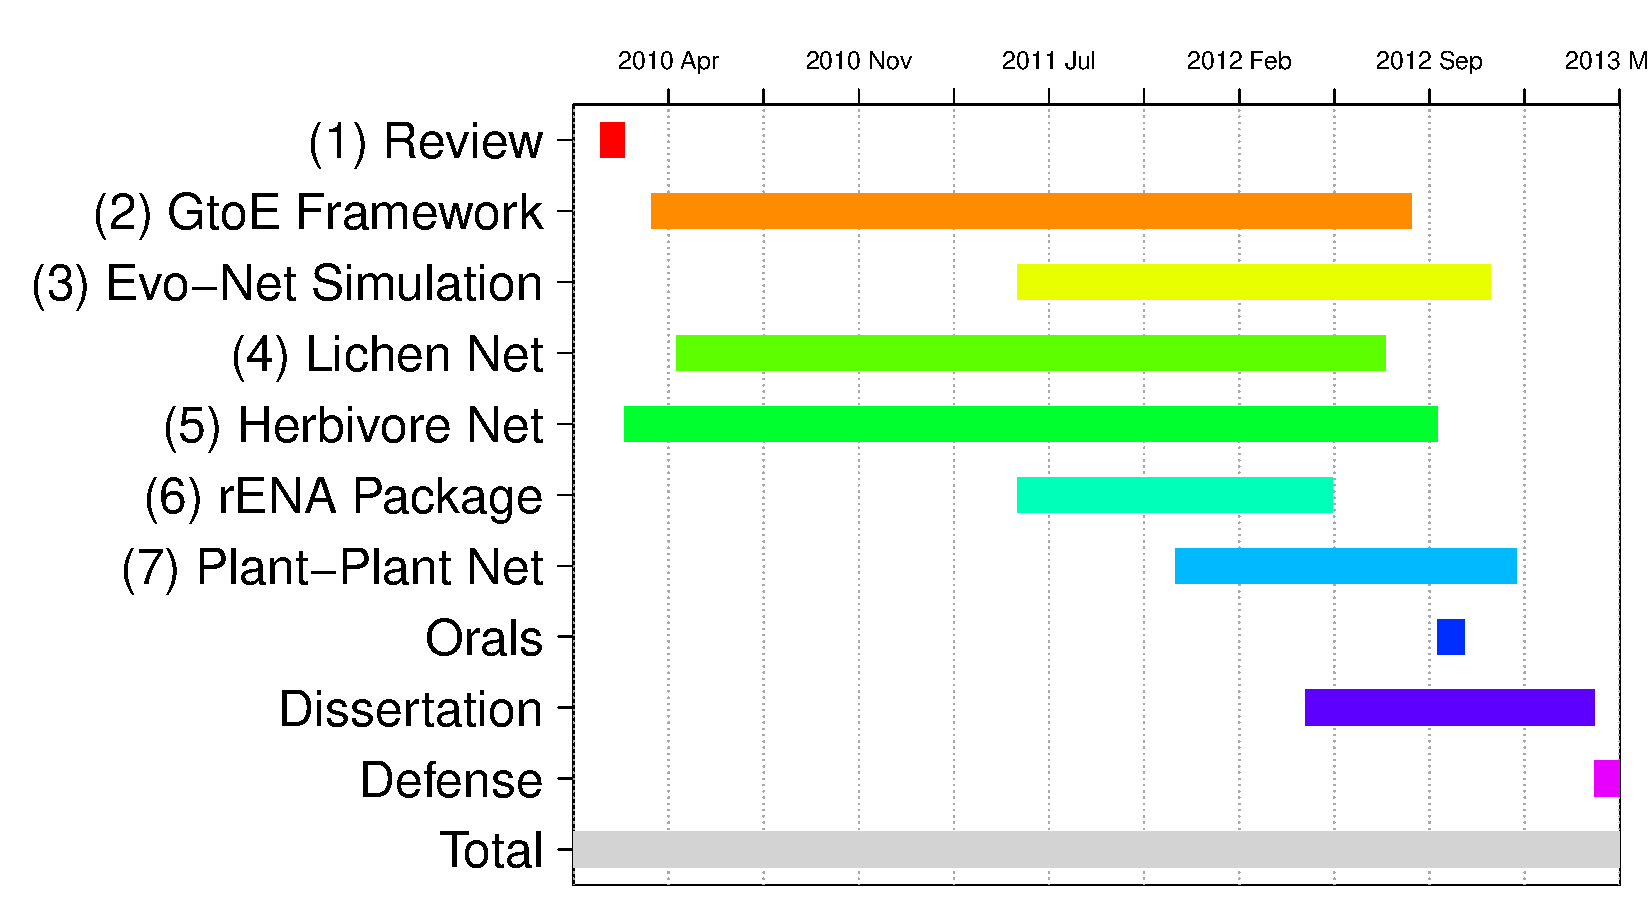
\includegraphics{committee_meeting-001}

%% \subsection{Post-Doc Goal}
%% \begin{itemize}
%% \item 
%% \end{itemize}

%% \subsection{Contingency Plan}
%% \begin{itemize}
%% \item 
%% \end{itemize}

\section{Requirements}

\subsection{Forms/Paperwork}

\begin{itemize}
\item \textbf{April 2012} Assessment, prospectus review and course plan approval
  \subitem Bio form 5 - PhD Program Form
  \subitem Bio form 10 - Progress/Funding Assessment
  \subitem Bio form 13 - Teaching requirement documentation
  \subitem Bio form 14 - Scientific paper presentation documentation
%\item \textbf{Oct 2012} Grant and written exam approval
\item \textbf{October 2012} Prospectus defense and oral exam
  \subitem Bio form 7 - Written exam results
  \subitem Bio form 10 - Progress/Funding Assessment
  \subitem Bio form 8 - Oral exam results REPORT
  \subitem Bio form 8.11a - Oral exam assessment/questionaire
  \subitem Bio form 9 - Prospectus approval form
  \subitem Bio form 11 - Oral exam results
  \subitem Bio form 10 - Progress/Funding Assessment
\item \textbf{May 2013} Final dissertation defense
  \subitem Dissertation draft
  \subitem Dissertation Defense Scheduling Form
  \subitem Graduate college final oral exam form (can only be accessed
  by advisor)
\end{itemize}

\section{References}

%%Activate for bibtex vibliography

\bibliographystyle{plain}
\bibliography{/Users/Aeolus/Documents/bibtex/biblib}


\end{document}  


